\section{Revisão de controladores no \texorpdfstring{plano $ s $}{plano-s} pelo LGR}

\begin{frame}{Introdução}
\begin{block}{Especificações no domínio do tempo}
\begin{itemize}
    \item O desempenho de um sistema de controle pode ser especificado utilizando certas métricas de desempenho.
    \item Geralmente, tais métricas são traduzidas em termos de \textbf{localização de  polos dominantes do sistema em malha fechada}. 
    \item Saber determinar regiões viáveis para tais polos a fim de garantir o desempenho esperado é fundamental em técnicas de projeto.
\end{itemize}
\end{block}
\end{frame}

\begin{frame}{Introdução}
\begin{block}{Projeto de sistemas de controle}
\begin{itemize}
    \item Na construção de um sistema de controle, uma modificação adequada na dinâmica da \textbf{planta} pode ser uma maneira simples de atender às especificações de desempenho. Isso, no entanto, pode \textbf{não ser possível} em muitas situações práticas porque a planta pode ser fixa e não ser passível de modificações.
    \item Nesses casos, devemos ajustar \textbf{outros parâmetros} que não aqueles da planta fixa.
\end{itemize}
\end{block}
\end{frame}

\begin{frame}{Introdução}
\begin{block}{Abordagem do LGR no projeto de sistemas de controle}
\begin{itemize}
    \item Na prática, o gráfico do \textbf{Lugar Geométrico das Raízes (LGR)} de um sistema pode indicar que o desempenho desejado não pode ser atingido simplesmente com o ajuste de ganho. Torna-se então necessário remodelar os lugares das raízes para atender às especificações de desempenho.
    \item Os problemas de projeto, portanto, tornam-se aqueles de melhorar o desempenho do sistema por meio da inclusão de um \textbf{compensador} (\textit{controlador}). A compensação de um sistema de controle fica reduzida ao projeto de um filtro cujas características tendem a compensar as características indesejáveis e inalteráveis da planta.
\end{itemize}
\end{block}
\end{frame}

\begin{frame}{Introdução}
\centering

\scalebox{0.8}{

\tikzset{every picture/.style={line width=0.75pt}} %set default line width to 0.75pt        

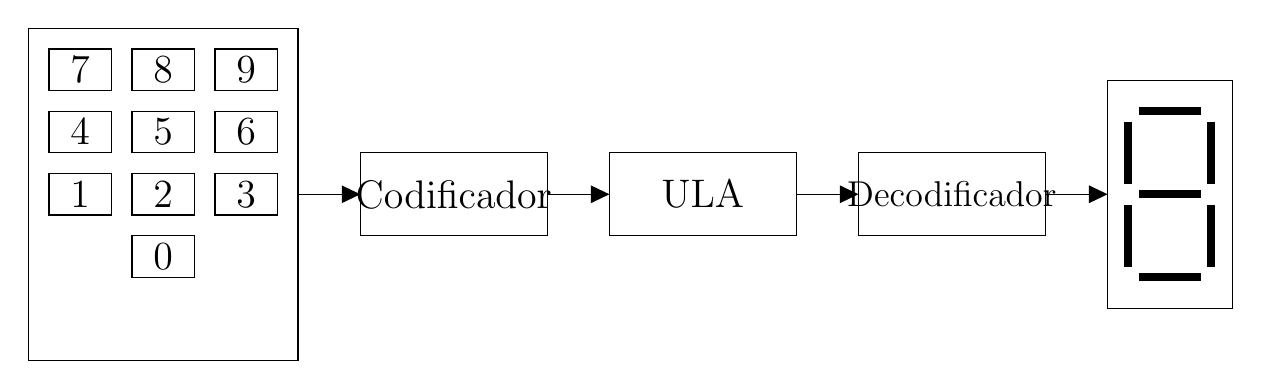
\begin{tikzpicture}[x=0.75pt,y=0.75pt,yscale=-1,xscale=1]
%uncomment if require: \path (0,300); %set diagram left start at 0, and has height of 300

%Shape: Rectangle [id:dp8798188650405219] 
\draw   (30,50) -- (160,50) -- (160,210) -- (30,210) -- cycle ;
%Shape: Rectangle [id:dp593444354888008] 
\draw   (40,60) -- (70,60) -- (70,80) -- (40,80) -- cycle ;
%Shape: Rectangle [id:dp4412846627526852] 
\draw   (80,60) -- (110,60) -- (110,80) -- (80,80) -- cycle ;
%Shape: Rectangle [id:dp2343273962035186] 
\draw   (120,60) -- (150,60) -- (150,80) -- (120,80) -- cycle ;
%Shape: Rectangle [id:dp05777918912875246] 
\draw   (40,90) -- (70,90) -- (70,110) -- (40,110) -- cycle ;
%Shape: Rectangle [id:dp9955010424516375] 
\draw   (80,90) -- (110,90) -- (110,110) -- (80,110) -- cycle ;
%Shape: Rectangle [id:dp24021539717259266] 
\draw   (120,90) -- (150,90) -- (150,110) -- (120,110) -- cycle ;
%Shape: Rectangle [id:dp36169684584711925] 
\draw   (40,120) -- (70,120) -- (70,140) -- (40,140) -- cycle ;
%Shape: Rectangle [id:dp7232437677097003] 
\draw   (80,120) -- (110,120) -- (110,140) -- (80,140) -- cycle ;
%Shape: Rectangle [id:dp6884539525496838] 
\draw   (120,120) -- (150,120) -- (150,140) -- (120,140) -- cycle ;
%Shape: Rectangle [id:dp9961423077173726] 
\draw   (80,150) -- (110,150) -- (110,170) -- (80,170) -- cycle ;
%Shape: Rectangle [id:dp6643057105712631] 
\draw   (190,110) -- (280,110) -- (280,150) -- (190,150) -- cycle ;
%Shape: Rectangle [id:dp7094011053258715] 
\draw   (550,75) -- (610,75) -- (610,185) -- (550,185) -- cycle ;
%Shape: Rectangle [id:dp2693438921699036] 
\draw   (310,110) -- (400,110) -- (400,150) -- (310,150) -- cycle ;
%Shape: Rectangle [id:dp3654960401722005] 
\draw   (430,110) -- (520,110) -- (520,150) -- (430,150) -- cycle ;
%Straight Lines [id:da6667328032348829] 
\draw    (160,130) -- (188,130) ;
\draw [shift={(190,130)}, rotate = 180] [fill={rgb, 255:red, 0; green, 0; blue, 0 }  ][line width=0.75]  [draw opacity=0] (8.93,-4.29) -- (0,0) -- (8.93,4.29) -- cycle    ;

%Straight Lines [id:da5165651690517046] 
\draw    (280,130) -- (308,130) ;
\draw [shift={(310,130)}, rotate = 180] [fill={rgb, 255:red, 0; green, 0; blue, 0 }  ][line width=0.75]  [draw opacity=0] (8.93,-4.29) -- (0,0) -- (8.93,4.29) -- cycle    ;

%Straight Lines [id:da17751850693095572] 
\draw    (400,130) -- (428,130) ;
\draw [shift={(430,130)}, rotate = 180] [fill={rgb, 255:red, 0; green, 0; blue, 0 }  ][line width=0.75]  [draw opacity=0] (8.93,-4.29) -- (0,0) -- (8.93,4.29) -- cycle    ;

%Straight Lines [id:da4998570413390182] 
\draw [color={rgb, 255:red, 0; green, 0; blue, 0 }  ,draw opacity=1 ][line width=3]    (560,95) -- (560,125) ;


%Straight Lines [id:da05287212083080073] 
\draw [color={rgb, 255:red, 0; green, 0; blue, 0 }  ,draw opacity=1 ][line width=3]    (600,95) -- (600,125) ;


%Straight Lines [id:da9146969001147236] 
\draw [color={rgb, 255:red, 0; green, 0; blue, 0 }  ,draw opacity=1 ][line width=3]    (560,135) -- (560,165) ;


%Straight Lines [id:da37610179690179124] 
\draw [color={rgb, 255:red, 0; green, 0; blue, 0 }  ,draw opacity=1 ][line width=3]    (600,135) -- (600,165) ;


%Straight Lines [id:da2798262228013664] 
\draw [color={rgb, 255:red, 0; green, 0; blue, 0 }  ,draw opacity=1 ][line width=3]    (595,130) -- (565,130) ;


%Straight Lines [id:da15184615547446478] 
\draw [color={rgb, 255:red, 0; green, 0; blue, 0 }  ,draw opacity=1 ][line width=3]    (595,90) -- (565,90) ;


%Straight Lines [id:da20609816632014244] 
\draw [color={rgb, 255:red, 0; green, 0; blue, 0 }  ,draw opacity=1 ][line width=3]    (595,170) -- (565,170) ;


%Straight Lines [id:da16937059284664002] 
\draw    (520,130) -- (548,130) ;
\draw [shift={(550,130)}, rotate = 180] [fill={rgb, 255:red, 0; green, 0; blue, 0 }  ][line width=0.75]  [draw opacity=0] (8.93,-4.29) -- (0,0) -- (8.93,4.29) -- cycle    ;


% Text Node
\draw (135,70) node   {\Large $9$};
% Text Node
\draw (95,70) node   {\Large $8$};
% Text Node
\draw (55,70) node   {\Large $7$};
% Text Node
\draw (135,100) node   {\Large $6$};
% Text Node
\draw (135,130) node   {\Large $3$};
% Text Node
\draw (95,160) node   {\Large $0$};
% Text Node
\draw (95,130) node   {\Large $2$};
% Text Node
\draw (95,100) node   {\Large $5$};
% Text Node
\draw (55,100) node   {\Large $4$};
% Text Node
\draw (55,130) node   {\Large $1$};
% Text Node
\draw (235,130) node  [align=left] {\Large Codificador};
% Text Node
\draw (355,130) node  [align=left] {\Large ULA};
% Text Node
\draw (475,130) node [scale=0.9] [align=left] {\Large Decodificador};


\end{tikzpicture}
}

\vspace{1cm}

\begin{block}{Forma padrão}
	\[ \dfrac{C(s)}{R(s)}=G(s)=\dfrac{\omega_n^{2}}{s^{2}+2\zeta\omega_n s+\omega_n^{2}} \]
\end{block}
\end{frame}


\begin{frame}{Introdução}
\begin{minipage}[c]{0.45\linewidth}
	\centering
	
	\vspace{-1.6cm}
	\scalebox{0.8}{\deftkzbds
	
\begin{tikzpicture}[auto, node distance=2cm,>=Latex]
	
	\node [input, name=input] {};
	
	\node [coordinate, right=of input] (junction) {};
	\draw (input) -- node[near start] {$E(z)$} (junction);
	
	\node [block, right=of junction] (ei) {$ C_i(z) $};
	\node [block, above=of ei] (kp) {$ C_p(z) $};
	\node [block, below=of ei] (cd) {$ C_d(z) $};
	
	\draw [->] (junction) -- (ei);
	\draw [->] (junction) |- (kp);
	\draw [->] (junction) |- (cd);
	
	\node [sum, right=2cm of ei] (sum) {$ \phantom{\sum} $};
	\draw (sum) ++(-8pt,-8pt) -- ++(16pt,16pt) ++(-16pt,0pt) -- +(16pt,-16pt);
	
	\draw [<-] (sum) -- node[very near start, above] {$ + $} (ei);
	\draw [<-] (sum) |- node[very near start, right] {$ + $} (kp);
	\draw [<-] (sum) |- node[very near start, left] {$ + $} (cd);
	
	\node [output, right=of sum] (output) {};
	\draw [->] (sum) -- node[near end] {$ U(z) $} (output);
\end{tikzpicture}}
	
	Subamortecido
\end{minipage}
\hfill
\begin{minipage}[c]{0.45\linewidth}
	\centering
	
	\scalebox{0.8}{%\begin{tikzpicture}[scale=1.5,>=latex, every node/.style={inner sep=2pt}]
%	
%	%\draw[pattern=north west lines, draw=mWhite] (0cm,0cm) circle(1cm);
%
%	\draw[dashed] (0cm,0cm) circle(1cm);
%	
%    % draw the coordinates
%    \draw[->, fill=white] (-1.5cm,0cm) -- (1.5cm,0cm) node[right=2pt] {$\Re(z)$};
%    \draw[->, fill=white] (0cm,-1.5cm) -- (0cm,1.5cm) node[above=2pt] {$\Im(z)$};
%    
%    \draw[->] (0,0) -- (45:1) node[right=2pt] {$ r=1 $};
%    
%    \draw[] (-1.4,0) ++(-2pt,-2pt) -- ++(4pt,4pt) ++(-4pt,0pt) -- ++(4pt,-4pt) +(-2pt,2pt) node[below=2pt, xshift=-3pt] {$ -1,4 $};
%    
%    \draw[fill=white] (-0.25,0) circle (1pt) node[below=2pt, xshift=-3pt] {$ -0,25 $};
%    
%    \draw[fill=white] (0,0) circle (1pt) node[below right=2pt] {$ 0 $};
%    
%    \draw[] (0.6,0) ++(-2pt,-2pt) -- ++(4pt,4pt) ++(-4pt,0pt) -- ++(4pt,-4pt) +(-2pt,2pt) node[below=2pt] {$ 0,6 $};
%\end{tikzpicture}


\begin{tikzpicture}[scale=1.5,>=latex, every node/.style={inner sep=2pt}]

\draw[pattern=south east lines, draw=mWhite] (0cm,0cm) circle(1.4cm);

\draw[dashed] (0cm,0cm) circle(1.4cm);

\draw[dashed, fill=white] (0cm,0cm) circle(0.6cm);

% draw the coordinates
\draw[->, fill=white] (-2cm,0cm) -- (2cm,0cm) node[right=2pt,fill=white] {$\Re(z)$};
\draw[->, fill=white] (0cm,-2cm) -- (0cm,2cm) node[above=2pt,fill=white] {$\Im(z)$};

%\draw[fill=black] (-1.4,0) ++(-2pt,-2pt) -- ++(4pt,4pt) ++(-4pt,0pt) -- ++(4pt,-4pt) +(-2pt,2pt) node[below left=2pt] {$ -1,4 $};

\node[below left=2pt] at (-1.4,0) {$ -1,4 $};

%    \draw[fill=black] (-0.6,0) circle (1pt) node[below=2pt,fill=mWhite] {$ -0,6 $};

%\draw[fill=black] (0.6,0) ++(-2pt,-2pt) -- ++(4pt,4pt) ++(-4pt,0pt) -- ++(4pt,-4pt) +(-2pt,2pt) node[below left=2pt] {$ 0,6 $};

\node[below left=2pt] at (0.6,0) {$ 0,6 $};

%    \draw[fill=black] (1.4,0) circle (1pt) node[below=2pt,fill=mWhite] {$ 1,4$};

	\draw[->,line width=1.2pt,white] (0,0) -- (45:1);
	\draw[->,thick] (0,0) -- (45:1) node[left,rotate=45,near start,below,xshift=2pt,yshift=1pt] {\tiny$ r=1 $};
	
	\draw[line width=1.2pt,white] (0cm,0cm) circle(1cm);
	\draw[densely dashed,thick] (0cm,0cm) circle(1cm);
\end{tikzpicture}}
	
	Criticamente amortecido
\end{minipage}

\end{frame}


\begin{frame}{Introdução}
\begin{block}{Definições}
	À medida que aumenta $ \zeta $ a resposta será muito \textbf{lenta}, mas tem erro \textbf{menor}.
	
	\vspace{1cm}
	
	\begin{minipage}{0.45\linewidth}
		\centering
		
		\scalebox{0.7}{\begin{tikzpicture}[scale=1.5,>=latex, every node/.style={inner sep=2pt}]
	
	\draw[pattern=south east lines, draw=mWhite] (0cm,0cm) circle(1.4cm);

	\draw[dashed] (0cm,0cm) circle(1.4cm);

	\draw[dashed, fill=mWhite] (0cm,0cm) circle(0.6cm);
	
    % draw the coordinates
    \draw[->, fill=mWhite] (-2cm,0cm) -- (2cm,0cm) node[right=2pt,fill=mWhite] {$\Re(z)$};
    \draw[->, fill=mWhite] (0cm,-2cm) -- (0cm,2cm) node[above=2pt,fill=mWhite] {$\Im(z)$};
    
    \draw[fill=black] (-1.4,0) ++(-2pt,-2pt) -- ++(4pt,4pt) ++(-4pt,0pt) -- ++(4pt,-4pt) +(-2pt,2pt) node[below left=2pt] {$ -1,4 $};
    
%    \draw[fill=black] (-0.6,0) circle (1pt) node[below=2pt,fill=mWhite] {$ -0,6 $};
    
    \draw[fill=black] (0.6,0) ++(-2pt,-2pt) -- ++(4pt,4pt) ++(-4pt,0pt) -- ++(4pt,-4pt) +(-2pt,2pt) node[below left=2pt] {$ 0,6 $};
    
%    \draw[fill=black] (1.4,0) circle (1pt) node[below=2pt,fill=mWhite] {$ 1,4$};

%	\draw[->] (0,0) -- (45:1) node[left] {$ r=1 $};
\end{tikzpicture}}
	\end{minipage}
	\hfill
	\begin{minipage}{0.45\linewidth}
		\begin{align*}
		T_p&=\dfrac{\pi}{\omega_d}\\
		T_r&=\dfrac{\pi-\theta}{\omega_d}\, , \, \theta=\tg^{-1}\dfrac{\omega_d}{\zeta\omega_n}\\
		M_p&=\text{e}^{-\pi}\left( \dfrac{\zeta}{\sqrt{1-\zeta^{2}}} \right)\\
		T_s&=\dfrac{4}{\zeta\omega_n}(2\%) 
		\end{align*}
	\end{minipage}
\end{block}
\end{frame}


\begin{frame}{Controlador avanço de fase}
\begin{block}{Características}
\begin{itemize}
	\item Melhora a resposta \textbf{transitória}.
	\item Torna o sistema \textbf{estável}.
\end{itemize}

\vspace{0.5cm}

\begin{minipage}{0.45\linewidth}
\centering

\scalebox{1}{\begin{tikzpicture}
\draw[->] (-2,0) -- (1,0);
\draw[->] (0,-0.5) -- (0,1.5);

\draw (-1.5,0) node[below=2pt] {$ -\dfrac{1}{\alpha T} $} ++(-2pt,-2pt) -- ++(4pt,4pt) ++(-4pt,0pt) -- +(4pt,-4pt);

\draw[fill=mWhite] (-0.5,0) circle (1.5pt) node[below=2pt] {$ -\dfrac{1}{T} $};
\end{tikzpicture}}
\end{minipage}
\hfill
\begin{minipage}{0.45\linewidth}
\[ G_c(s)=K_c\cdot\dfrac{s+\dfrac{1}{T}}{s+\dfrac{1}{\alpha T}} \]
$$0 < \alpha < 1$$
\end{minipage}
\vspace{0.5cm}
\begin{itemize}
	\item Considere que $\delta_1$ é o ângulo do zero com um ponto de teste no eixo $j\omega$, e que $\delta_2$ é o ângulo do polo com um ponto de teste no eixo $j\omega$.
	\item Como $\delta_1 > \delta_2$, temos que $\delta_1 - \delta_2 > 0$; daí o nome \textbf{avanço de fase}.
\end{itemize}
\end{block}
\end{frame}


\begin{frame}{Controlador avanço de fase}
\begin{block}{Passos}
\begin{enumerate}
\item A partir das especificações de desempenho, determine os \textbf{polos desejados dominantes} em malha fechada.
\item Encontre o ângulo de \textbf{avanço} $ \phi $ para que os polos pertençam ao LGR.
\item Determine $ \alpha $ e $ T $, isto é, a \textbf{posição do polo e zero} com base na deficiência angular (de modo que o compensador complete o ângulo $ \phi $ necessário).
\item Encontre $ K_c $ usando \textbf{condição de módulo}.
\end{enumerate}
\end{block}
\end{frame}


\begin{frame}{Controlador avanço de fase - Exemplo \#01}
\begin{block}{Problema}
Deseja-se $ \omega_n=\SI{4}{\radian\per\second} $ e $ \zeta $ igual do sistema em malha fechada sem compensação.
\end{block}

\vspace{1cm}

\centering

\scalebox{0.9}{\deftkzbds
	
	\begin{tikzpicture}[auto, node distance=2cm,>=Latex]
		% We start by placing the blocks
		\node [input] (input) {};
		\node [block, right=of input, xshift=0cm] (SH) {S/H};
		\node [block, right=of SH] (quantizer) {quantizador};
		\node [output, right =of quantizer, xshift=0cm] (output) {};
		\node [input, below= of SH, xshift=2cm] (clock) {};
		\node [above=1cm, name=midp, node distance=1pt, inner sep=1pt, fill=black, circle, draw] at (clock) {};
		
		\node [above] at (input) {entrada};
		\node [above] at (output) {saída};
		
		\draw [->] (input) -- (SH);
		\draw [->] (quantizer) -- (output);
		\draw [->] (SH) -- (quantizer);
		\draw [] (quantizer) |- (midp);
		\draw [->] (midp) -| (SH);
		\draw (midp) -- (clock) node[below=0pt] {clock};
		
		\draw [<-] (SH) -- +(0,1.5) node[above, name=alias] {\textit{aliasing}};
		\node [above=5pt] at (alias) {$ \omega_s>2\omega_c $};
		
		\draw [loosely dashed] ($(input)+(1,1)$) rectangle ($(output)+(-1,-2)$) node[yshift=7pt, xshift=-13pt] {A/D};
		
		\draw [<-, dashed] (quantizer.north) -- +(3,1) node[right, text width=4cm, align=center, name=txt1] {efeito de quantização (limitação ou recurso finito)};
		
		\draw [->] (txt1) -- +(0,-1) node[align=center, below, name=txt2] {truncamento $\left[q\right]$};
		
		\draw [->] (txt2) -- +(0,-1) node[align=center, below] {\textbf{erro}};
		\end{tikzpicture}}
\end{frame}

\begin{frame}{Controlador avanço de fase - Exemplo \#01}
	\begin{block}{Resolução}
		\begin{enumerate}
			\item 
			\[ G(s)=\dfrac{4}{s^{2}+2s+4}=\dfrac{\omega_n^{2}}{s^{2}+2\zeta\omega_n s+\omega_n^{2}}\rightarrow \, \begin{aligned}
			\omega_n&=\SI{2}{\radian\per\second}\\
			\zeta&=0.5
			\end{aligned} \]
			\begin{align*}
			\text{Polos desejados em }s&=-\zeta\omega_n\pm j\omega_n\sqrt{1-\zeta^{2}}\\
			s&=-2\pm j3,46
			\end{align*}
			%	\setcounter{enumi}{4}
		\end{enumerate}
	\end{block}
\end{frame}

\begin{frame}{Controlador avanço de fase - Exemplo \#01}
\centerline{\includegraphics[width=0.8\linewidth]{Figuras/Ch09/fig1.png}}
\end{frame}

\begin{frame}{Controlador avanço de fase - Exemplo \#01}
\centerline{\includegraphics[width=0.8\linewidth]{Figuras/Ch09/fig2.png}}
\end{frame}


\begin{frame}{Controlador avanço de fase - Exemplo \#01}
\begin{block}{Resolução}
\begin{enumerate}
	\setcounter{enumi}{1}
	\item 
\end{enumerate}
\begin{minipage}{0.35\linewidth}
	\centering
	
	\scalebox{0.7}{\begin{tikzpicture}[y=0.75cm]
\draw[->] (-3,0) -- (1.5,0) node[right=2pt] {$ \sigma $};
\draw[->] (0,-4.5) -- (0,4.5) node[above=2pt] {$ j \omega $};

\draw[-{Latex[width=2pt, length=5pt]}] (-2,0) -- (-2,3.46);

\draw[dashed] (0,3.46) -- (-2,3.46);
\draw (-0.2,3.46) -- (0.2,3.46) node[right] {$ \num{3,46} $};

\draw[-{Latex[width=2pt, length=5pt]}] (0,0) -- (-2,3.46);
\draw (0,0) ++(-2pt,-2pt) -- ++(4pt,4pt) ++(-4pt,0pt) -- +(4pt,-4pt);

\draw (-0.2,-3.46) -- (0.2, -3.46) node[right] {$ \num{-3,46} $};

\draw[dashed] (-2,0) |- (0,-3.46);

\fill (-2,3.46) circle (1.2pt);

\node[below=2pt, fill=mWhite, inner sep=1pt] at (-2,0) {$ -2 $};

\draw[->] (0.5,0) arc (0:120:0.5cm) node[midway, above right=-3pt] {$ \gamma $};

\draw[->] (-1.7,0) arc (0:90:0.3cm) node[midway, above right=-3pt] {$ \alpha $};

\draw (-0.5,0) arc(180:120:0.5cm) node[left,midway] {$ \theta $};

\draw (-2,0) ++(-2pt,-2pt) -- ++(4pt,4pt) ++(-4pt,0pt) -- +(4pt,-4pt);

\end{tikzpicture}}
\end{minipage}
\hfill
\begin{minipage}{0.6\linewidth}
	\begin{align*}
	\gamma&=\ang{180}-\tg^{-1}\left( \dfrac{\num{3,46}}{2}\right)=\ang{120}\\
	\alpha&=\ang{90}\\
	\sum \text{Ângulos}&=\ang{0}-\left( \ang{120}+\ang{90}\right) =\ang{-210}
	\end{align*}
\end{minipage}

Pela condição de ângulo ($ \pm180(2k+1) $), \textbf{$ \bm{\phi=}\ang{30} $}, ângulo de avanço.
\end{block}
\end{frame}


\begin{frame}{Controlador avanço de fase - Exemplo \#01}
\begin{block}{Resolução}
\begin{enumerate}
	\setcounter{enumi}{2}
	\item 
\end{enumerate}

\centering

\scalebox{0.8}{\tikzset{every picture/.style={line width=0.75pt}} %set default line width to 0.75pt  

\begin{tikzpicture}[x=0.75pt,y=0.75pt,yscale=-1,xscale=1]

%uncomment if require: \path (0,300); %set diagram left start at 0, and has height of 300

%Straight Lines [id:da8305438567766523] 
\draw    (200.27,190.67) -- (365.77,190.67) ;
\draw [shift={(367.77,190.67)}, rotate = 180] [color={rgb, 255:red, 0; green, 0; blue, 0 }  ][line width=0.75]    (10.93,-3.29) .. controls (6.95,-1.4) and (3.31,-0.3) .. (0,0) .. controls (3.31,0.3) and (6.95,1.4) .. (10.93,3.29)   ;

%Shape: Circle [id:dp5343795865479193] 
\draw  [fill={rgb, 255:red, 255; green, 255; blue, 255 }  ,fill opacity=1 ] (207.97,191.08) .. controls (207.97,189.75) and (209.05,188.67) .. (210.38,188.67) .. controls (211.72,188.67) and (212.8,189.75) .. (212.8,191.08) .. controls (212.8,192.42) and (211.72,193.5) .. (210.38,193.5) .. controls (209.05,193.5) and (207.97,192.42) .. (207.97,191.08) -- cycle ;
%Shape: Circle [id:dp9958561748525927] 
\draw  [fill={rgb, 255:red, 255; green, 255; blue, 255 }  ,fill opacity=1 ] (227.57,190.68) .. controls (227.57,189.35) and (228.65,188.27) .. (229.98,188.27) .. controls (231.32,188.27) and (232.4,189.35) .. (232.4,190.68) .. controls (232.4,192.02) and (231.32,193.1) .. (229.98,193.1) .. controls (228.65,193.1) and (227.57,192.02) .. (227.57,190.68) -- cycle ;
%Straight Lines [id:da3574860753882376] 
\draw    (250.58,108.68) -- (250.58,190.28) ;


%Shape: Circle [id:dp04408180627185376] 
\draw  [fill={rgb, 255:red, 255; green, 255; blue, 255 }  ,fill opacity=1 ] (248.17,108.68) .. controls (248.17,107.35) and (249.25,106.27) .. (250.58,106.27) .. controls (251.92,106.27) and (253,107.35) .. (253,108.68) .. controls (253,110.02) and (251.92,111.1) .. (250.58,111.1) .. controls (249.25,111.1) and (248.17,110.02) .. (248.17,108.68) -- cycle ;
%Straight Lines [id:da7712579502140393] 
\draw    (270.58,129.5) -- (270.58,190.28) ;


%Shape: Circle [id:dp4215879501304003] 
\draw  [fill={rgb, 255:red, 255; green, 255; blue, 255 }  ,fill opacity=1 ] (268.17,129.5) .. controls (268.17,128.17) and (269.25,127.08) .. (270.58,127.08) .. controls (271.92,127.08) and (273,128.17) .. (273,129.5) .. controls (273,130.83) and (271.92,131.92) .. (270.58,131.92) .. controls (269.25,131.92) and (268.17,130.83) .. (268.17,129.5) -- cycle ;
%Straight Lines [id:da39800912811539835] 
\draw    (290.58,149.5) -- (290.58,190.28) ;


%Straight Lines [id:da15358320586768315] 
\draw    (311.08,171.5) -- (311.08,190.78) ;


%Shape: Circle [id:dp9326128099979845] 
\draw  [fill={rgb, 255:red, 255; green, 255; blue, 255 }  ,fill opacity=1 ] (288.17,149.5) .. controls (288.17,148.17) and (289.25,147.08) .. (290.58,147.08) .. controls (291.92,147.08) and (293,148.17) .. (293,149.5) .. controls (293,150.83) and (291.92,151.92) .. (290.58,151.92) .. controls (289.25,151.92) and (288.17,150.83) .. (288.17,149.5) -- cycle ;
%Shape: Circle [id:dp7866868035269907] 
\draw  [fill={rgb, 255:red, 255; green, 255; blue, 255 }  ,fill opacity=1 ] (308.67,169.08) .. controls (308.67,167.75) and (309.75,166.67) .. (311.08,166.67) .. controls (312.42,166.67) and (313.5,167.75) .. (313.5,169.08) .. controls (313.5,170.42) and (312.42,171.5) .. (311.08,171.5) .. controls (309.75,171.5) and (308.67,170.42) .. (308.67,169.08) -- cycle ;

% Text Node
\draw (334,178.5) node   {$\dotsc $};
% Text Node
\draw (371.5,200) node   {$n$};
% Text Node
\draw (251.5,200) node   {$0$};
% Text Node
\draw (271.5,200) node   {$1$};
% Text Node
\draw (292,200) node   {$2$};
% Text Node
\draw (312.5,200) node   {$3$};

\end{tikzpicture}}

\vspace{-0.5cm}

\[ \theta=\tg^{-1}\left( \dfrac{\num{3,46}}{2}\right) =\ang{60} \]
\end{block}
\end{frame}


\begin{frame}{Controlador avanço de fase - Exemplo \#01}
\begin{block}{Resolução}
\begin{enumerate}
	\setcounter{enumi}{2}
	\item 
\end{enumerate}
\begin{minipage}{0.5\linewidth}
	\centering
	
	\scalebox{0.8}{\tikzset{every picture/.style={line width=0.75pt}} %set default line width to 0.75pt  

\begin{tikzpicture}[x=0.75pt,y=0.75pt,yscale=-1,xscale=1]

%uncomment if require: \path (0,300); %set diagram left start at 0, and has height of 300

%Straight Lines [id:da8305438567766523] 
\draw    (200.27,190.67) -- (365.77,190.67) ;
\draw [shift={(367.77,190.67)}, rotate = 180] [color={rgb, 255:red, 0; green, 0; blue, 0 }  ][line width=0.75]    (10.93,-3.29) .. controls (6.95,-1.4) and (3.31,-0.3) .. (0,0) .. controls (3.31,0.3) and (6.95,1.4) .. (10.93,3.29)   ;

%Shape: Circle [id:dp5343795865479193] 
\draw  [fill={rgb, 255:red, 255; green, 255; blue, 255 }  ,fill opacity=1 ] (207.97,191.08) .. controls (207.97,189.75) and (209.05,188.67) .. (210.38,188.67) .. controls (211.72,188.67) and (212.8,189.75) .. (212.8,191.08) .. controls (212.8,192.42) and (211.72,193.5) .. (210.38,193.5) .. controls (209.05,193.5) and (207.97,192.42) .. (207.97,191.08) -- cycle ;
%Shape: Circle [id:dp9958561748525927] 
\draw  [fill={rgb, 255:red, 255; green, 255; blue, 255 }  ,fill opacity=1 ] (227.57,190.68) .. controls (227.57,189.35) and (228.65,188.27) .. (229.98,188.27) .. controls (231.32,188.27) and (232.4,189.35) .. (232.4,190.68) .. controls (232.4,192.02) and (231.32,193.1) .. (229.98,193.1) .. controls (228.65,193.1) and (227.57,192.02) .. (227.57,190.68) -- cycle ;
%Straight Lines [id:da3574860753882376] 
\draw    (250.58,108.68) -- (250.58,190.28) ;


%Shape: Circle [id:dp04408180627185376] 
\draw  [fill={rgb, 255:red, 255; green, 255; blue, 255 }  ,fill opacity=1 ] (248.17,108.68) .. controls (248.17,107.35) and (249.25,106.27) .. (250.58,106.27) .. controls (251.92,106.27) and (253,107.35) .. (253,108.68) .. controls (253,110.02) and (251.92,111.1) .. (250.58,111.1) .. controls (249.25,111.1) and (248.17,110.02) .. (248.17,108.68) -- cycle ;
%Straight Lines [id:da7712579502140393] 
\draw    (270.58,129.5) -- (270.58,190.28) ;


%Shape: Circle [id:dp4215879501304003] 
\draw  [fill={rgb, 255:red, 255; green, 255; blue, 255 }  ,fill opacity=1 ] (268.17,129.5) .. controls (268.17,128.17) and (269.25,127.08) .. (270.58,127.08) .. controls (271.92,127.08) and (273,128.17) .. (273,129.5) .. controls (273,130.83) and (271.92,131.92) .. (270.58,131.92) .. controls (269.25,131.92) and (268.17,130.83) .. (268.17,129.5) -- cycle ;
%Straight Lines [id:da39800912811539835] 
\draw    (290.58,149.5) -- (290.58,190.28) ;


%Straight Lines [id:da15358320586768315] 
\draw    (311.08,171.5) -- (311.08,190.78) ;


%Shape: Circle [id:dp9326128099979845] 
\draw  [fill={rgb, 255:red, 255; green, 255; blue, 255 }  ,fill opacity=1 ] (288.17,149.5) .. controls (288.17,148.17) and (289.25,147.08) .. (290.58,147.08) .. controls (291.92,147.08) and (293,148.17) .. (293,149.5) .. controls (293,150.83) and (291.92,151.92) .. (290.58,151.92) .. controls (289.25,151.92) and (288.17,150.83) .. (288.17,149.5) -- cycle ;
%Shape: Circle [id:dp7866868035269907] 
\draw  [fill={rgb, 255:red, 255; green, 255; blue, 255 }  ,fill opacity=1 ] (308.67,169.08) .. controls (308.67,167.75) and (309.75,166.67) .. (311.08,166.67) .. controls (312.42,166.67) and (313.5,167.75) .. (313.5,169.08) .. controls (313.5,170.42) and (312.42,171.5) .. (311.08,171.5) .. controls (309.75,171.5) and (308.67,170.42) .. (308.67,169.08) -- cycle ;

% Text Node
\draw (334,178.5) node   {$\dotsc $};
% Text Node
\draw (371.5,200) node   {$n$};
% Text Node
\draw (251.5,200) node   {$0$};
% Text Node
\draw (271.5,200) node   {$1$};
% Text Node
\draw (292,200) node   {$2$};
% Text Node
\draw (312.5,200) node   {$3$};

\end{tikzpicture}}
\end{minipage}
\hfill
\begin{minipage}{0.4\linewidth}
	\centering
	
	\scalebox{0.8}{\begin{tikzpicture}
\draw (0,0) -- node[midway, below] {$ \dfrac{1}{T} $} (2.2,0);

\draw (0,0) -- (75:2.69);

\draw (0.3,0) arc (0:75:0.3) node[midway, right] {$ \ang{75} $};

\draw (2.2,0) -- +(120:3) node[midway,right] {$ \omega_n $};

\draw (1.9,0) arc (180:120:0.3) node[midway, left, yshift=2pt] {$ \theta $};

\draw (0.7,2.6) +(-0.13,-0.48) arc (255:300:0.5) node[coordinate, name=B] {};

\draw[->] (B) +(-0.2,0.1) parabola bend (1,2.4) (1.2,2.5) node[above] {$ \dfrac{\ang{180}-\theta}{2}-\dfrac{\phi}{2}=\ang{45} $};
\end{tikzpicture}}
	
	\vspace{-0.5cm}
	\begin{align*}
	\dfrac{\omega_n}{\sen\ang{75}}&=\dfrac{1/T}{\sen\ang{45}}\\
	\dfrac{1}{T}&=\num{2,93}
	\end{align*}
\end{minipage}
\end{block}
\end{frame}


\begin{frame}{Controlador avanço de fase - Exemplo \#01}
\begin{block}{Resolução}
	\begin{enumerate}
	\setcounter{enumi}{2}
	\item 
\end{enumerate}
\begin{minipage}{0.5\linewidth}
	\centering
	
	\scalebox{0.8}{\tikzset{every picture/.style={line width=0.75pt}} %set default line width to 0.75pt  

\begin{tikzpicture}[x=0.75pt,y=0.75pt,yscale=-1,xscale=1]

%uncomment if require: \path (0,300); %set diagram left start at 0, and has height of 300

%Straight Lines [id:da8305438567766523] 
\draw    (200.27,190.67) -- (365.77,190.67) ;
\draw [shift={(367.77,190.67)}, rotate = 180] [color={rgb, 255:red, 0; green, 0; blue, 0 }  ][line width=0.75]    (10.93,-3.29) .. controls (6.95,-1.4) and (3.31,-0.3) .. (0,0) .. controls (3.31,0.3) and (6.95,1.4) .. (10.93,3.29)   ;

%Shape: Circle [id:dp5343795865479193] 
\draw  [fill={rgb, 255:red, 255; green, 255; blue, 255 }  ,fill opacity=1 ] (207.97,191.08) .. controls (207.97,189.75) and (209.05,188.67) .. (210.38,188.67) .. controls (211.72,188.67) and (212.8,189.75) .. (212.8,191.08) .. controls (212.8,192.42) and (211.72,193.5) .. (210.38,193.5) .. controls (209.05,193.5) and (207.97,192.42) .. (207.97,191.08) -- cycle ;
%Shape: Circle [id:dp9958561748525927] 
\draw  [fill={rgb, 255:red, 255; green, 255; blue, 255 }  ,fill opacity=1 ] (227.57,190.68) .. controls (227.57,189.35) and (228.65,188.27) .. (229.98,188.27) .. controls (231.32,188.27) and (232.4,189.35) .. (232.4,190.68) .. controls (232.4,192.02) and (231.32,193.1) .. (229.98,193.1) .. controls (228.65,193.1) and (227.57,192.02) .. (227.57,190.68) -- cycle ;
%Straight Lines [id:da3574860753882376] 
\draw    (250.58,108.68) -- (250.58,190.28) ;


%Shape: Circle [id:dp04408180627185376] 
\draw  [fill={rgb, 255:red, 255; green, 255; blue, 255 }  ,fill opacity=1 ] (248.17,108.68) .. controls (248.17,107.35) and (249.25,106.27) .. (250.58,106.27) .. controls (251.92,106.27) and (253,107.35) .. (253,108.68) .. controls (253,110.02) and (251.92,111.1) .. (250.58,111.1) .. controls (249.25,111.1) and (248.17,110.02) .. (248.17,108.68) -- cycle ;
%Straight Lines [id:da7712579502140393] 
\draw    (270.58,129.5) -- (270.58,190.28) ;


%Shape: Circle [id:dp4215879501304003] 
\draw  [fill={rgb, 255:red, 255; green, 255; blue, 255 }  ,fill opacity=1 ] (268.17,129.5) .. controls (268.17,128.17) and (269.25,127.08) .. (270.58,127.08) .. controls (271.92,127.08) and (273,128.17) .. (273,129.5) .. controls (273,130.83) and (271.92,131.92) .. (270.58,131.92) .. controls (269.25,131.92) and (268.17,130.83) .. (268.17,129.5) -- cycle ;
%Straight Lines [id:da39800912811539835] 
\draw    (290.58,149.5) -- (290.58,190.28) ;


%Straight Lines [id:da15358320586768315] 
\draw    (311.08,171.5) -- (311.08,190.78) ;


%Shape: Circle [id:dp9326128099979845] 
\draw  [fill={rgb, 255:red, 255; green, 255; blue, 255 }  ,fill opacity=1 ] (288.17,149.5) .. controls (288.17,148.17) and (289.25,147.08) .. (290.58,147.08) .. controls (291.92,147.08) and (293,148.17) .. (293,149.5) .. controls (293,150.83) and (291.92,151.92) .. (290.58,151.92) .. controls (289.25,151.92) and (288.17,150.83) .. (288.17,149.5) -- cycle ;
%Shape: Circle [id:dp7866868035269907] 
\draw  [fill={rgb, 255:red, 255; green, 255; blue, 255 }  ,fill opacity=1 ] (308.67,169.08) .. controls (308.67,167.75) and (309.75,166.67) .. (311.08,166.67) .. controls (312.42,166.67) and (313.5,167.75) .. (313.5,169.08) .. controls (313.5,170.42) and (312.42,171.5) .. (311.08,171.5) .. controls (309.75,171.5) and (308.67,170.42) .. (308.67,169.08) -- cycle ;

% Text Node
\draw (334,178.5) node   {$\dotsc $};
% Text Node
\draw (371.5,200) node   {$n$};
% Text Node
\draw (251.5,200) node   {$0$};
% Text Node
\draw (271.5,200) node   {$1$};
% Text Node
\draw (292,200) node   {$2$};
% Text Node
\draw (312.5,200) node   {$3$};

\end{tikzpicture}}
\end{minipage}
\hfill
\begin{minipage}{0.4\linewidth}
	\centering
	
	\scalebox{0.7}{

\tikzset{every picture/.style={line width=0.75pt}} %set default line width to 0.75pt        

\begin{tikzpicture}[x=0.75pt,y=0.75pt,yscale=-1,xscale=1]
%uncomment if require: \path (0,300); %set diagram left start at 0, and has height of 300

%Straight Lines [id:da8305438567766523] 
\draw    (200.27,190.67) -- (365.77,190.67) ;
\draw [shift={(367.77,190.67)}, rotate = 180] [color={rgb, 255:red, 0; green, 0; blue, 0 }  ][line width=0.75]    (10.93,-3.29) .. controls (6.95,-1.4) and (3.31,-0.3) .. (0,0) .. controls (3.31,0.3) and (6.95,1.4) .. (10.93,3.29)   ;

%Shape: Circle [id:dp5343795865479193] 
\draw  [fill={rgb, 255:red, 255; green, 255; blue, 255 }  ,fill opacity=1 ] (347.47,190.58) .. controls (347.47,189.25) and (348.55,188.17) .. (349.88,188.17) .. controls (351.22,188.17) and (352.3,189.25) .. (352.3,190.58) .. controls (352.3,191.92) and (351.22,193) .. (349.88,193) .. controls (348.55,193) and (347.47,191.92) .. (347.47,190.58) -- cycle ;
%Shape: Circle [id:dp9958561748525927] 
\draw  [fill={rgb, 255:red, 255; green, 255; blue, 255 }  ,fill opacity=1 ] (328.07,190.68) .. controls (328.07,189.35) and (329.15,188.27) .. (330.48,188.27) .. controls (331.82,188.27) and (332.9,189.35) .. (332.9,190.68) .. controls (332.9,192.02) and (331.82,193.1) .. (330.48,193.1) .. controls (329.15,193.1) and (328.07,192.02) .. (328.07,190.68) -- cycle ;
%Straight Lines [id:da3574860753882376] 
\draw    (250.57,272.59) -- (250.57,191.28) ;


%Shape: Circle [id:dp04408180627185376] 
\draw  [fill={rgb, 255:red, 255; green, 255; blue, 255 }  ,fill opacity=1 ] (248.17,272.59) .. controls (248.17,273.92) and (249.24,275) .. (250.57,275) .. controls (251.9,275) and (252.98,273.92) .. (252.98,272.59) .. controls (252.98,271.26) and (251.9,270.18) .. (250.57,270.18) .. controls (249.24,270.18) and (248.17,271.26) .. (248.17,272.59) -- cycle ;
%Straight Lines [id:da7712579502140393] 
\draw    (270.5,251.85) -- (270.5,191.28) ;


%Shape: Circle [id:dp4215879501304003] 
\draw  [fill={rgb, 255:red, 255; green, 255; blue, 255 }  ,fill opacity=1 ] (268.1,251.85) .. controls (268.1,253.18) and (269.17,254.26) .. (270.5,254.26) .. controls (271.83,254.26) and (272.91,253.18) .. (272.91,251.85) .. controls (272.91,250.52) and (271.83,249.44) .. (270.5,249.44) .. controls (269.17,249.44) and (268.1,250.52) .. (268.1,251.85) -- cycle ;
%Straight Lines [id:da39800912811539835] 
\draw    (290.43,231.92) -- (290.43,191.28) ;


%Straight Lines [id:da15358320586768315] 
\draw    (310.86,210) -- (310.86,190.78) ;


%Shape: Circle [id:dp9326128099979845] 
\draw  [fill={rgb, 255:red, 255; green, 255; blue, 255 }  ,fill opacity=1 ] (288.02,231.92) .. controls (288.02,233.25) and (289.1,234.33) .. (290.43,234.33) .. controls (291.76,234.33) and (292.84,233.25) .. (292.84,231.92) .. controls (292.84,230.59) and (291.76,229.51) .. (290.43,229.51) .. controls (289.1,229.51) and (288.02,230.59) .. (288.02,231.92) -- cycle ;
%Shape: Circle [id:dp7866868035269907] 
\draw  [fill={rgb, 255:red, 255; green, 255; blue, 255 }  ,fill opacity=1 ] (308.45,212.41) .. controls (308.45,213.74) and (309.53,214.81) .. (310.86,214.81) .. controls (312.19,214.81) and (313.27,213.74) .. (313.27,212.41) .. controls (313.27,211.08) and (312.19,210) .. (310.86,210) .. controls (309.53,210) and (308.45,211.08) .. (308.45,212.41) -- cycle ;

% Text Node
\draw (224,203) node   {$\dotsc $};
% Text Node
\draw (371.5,197) node   {$n$};
% Text Node
\draw (310,180) node   {$-1$};
% Text Node
\draw (287,180) node   {$-2$};
% Text Node
\draw (265,180) node   {$-3$};
% Text Node
\draw (246,180) node   {$-4$};


\end{tikzpicture}
}
	
	\vspace{-0.5cm}
	\begin{align*}
	\dfrac{\omega_n}{\sen45^{\circ}}&=\dfrac{1/\alpha T}{\sen75^{\circ}}\\
	\dfrac{1}{\alpha T}&=\num{5,46}
	\end{align*}
\end{minipage}
\end{block}
\end{frame}


\begin{frame}{Controlador avanço de fase - Exemplo \#01}
\begin{block}{Resolução}
\begin{enumerate}
	\setcounter{enumi}{3}
	\item \begin{align*}
		G_c(s)G(s)&=\eval{\left| K_c\cdot\dfrac{s+\num{2,93}}{s+\num{5,46}}\cdot\dfrac{4}{s(s+2)}\right|}_{s=-2+j\num{3,46}}=1\Rightarrow\\
		\left| 4K_c\cdot\dfrac{\num{3,57}}{\num{4,85}\cdot4\cdot\num{3,46}} \right|&=1\Rightarrow K_c=\num{4,7}\\
		\Aboxed{G_c(s)&=\num{4,7}\cdot\dfrac{s+\num{2,93}}{s+\num{5,46}}}
	\end{align*}
\end{enumerate}
\end{block}
\end{frame}

\begin{frame}{Controlador avanço de fase - Exemplo \#01}
\centerline{\includegraphics[width=0.8\linewidth]{Figuras/Ch09/fig3.png}}
\end{frame}

\begin{frame}{Controlador avanço de fase - Exemplo \#01}
\centerline{\includegraphics[width=0.8\linewidth]{Figuras/Ch09/fig4.png}}
\end{frame}

\begin{frame}{Controlador avanço de fase - Exemplo \#01}
\centerline{\includegraphics[width=0.8\linewidth]{Figuras/Ch09/fig5.png}}
\end{frame}


\begin{frame}{Controlador avanço de fase - Exemplo \#02}
\begin{block}{Problema}
Deseja-se $T_s=\SI{1}{\second} $ e $ M_p = 5 \%$.
\end{block}

\vspace{1cm}

\centering

\scalebox{0.9}{\deftkzbds

\begin{tikzpicture}[auto, node distance=1.5cm,>=Latex]

\node [input, name=input] {};
\node [sum, right =of input, xshift=0.5cm] (pm) {$ \sum $};
\draw [draw,->] (input) -- node {$R(s)$} (pm);

\node [block, right =of pm, text width=2cm, align=center] (Gc) {$ \dfrac{1}{(s+1)(s+2)} $};
\draw [->] (pm) -- (Gc);

\node [output, right =of Gc] (output) {};
\draw [->] (Gc) -- node [name=outAr] {$C(s)$}(output);

\node [coordinate,below=1.5cm] at (Gc) (Hs) {};
\draw[->] (outAr) |- (Hs) -| node[pos=0.98, xshift=15pt] {$-$} node[pos=1.4, xshift=-4pt] {$+$} (pm);

\end{tikzpicture}}
\end{frame}


\begin{frame}{Controlador avanço de fase - Exemplo \#02}
\begin{block}{Resolução}
\begin{enumerate}
%	\setcounter{enumi}{3}
	\item \begin{align*}
	M_p&=5\%\Rightarrow \zeta\approx \num{0,7}\\
	T_s&=\dfrac{4}{\zeta \omega_n}\Rightarrow\omega_n\approx\SI{5,71}{\radian\per\second}
	\end{align*}
	\begin{align*}
			\text{Polos desejados em }s&=-\zeta\omega_n\pm j\omega_n\sqrt{1-\zeta^{2}}\\
			s&=-4\pm j4
	\end{align*}
\end{enumerate}
\end{block}
\end{frame}

\begin{frame}{Controlador avanço de fase - Exemplo \#02}
\centerline{\includegraphics[width=0.8\linewidth]{Figuras/Ch09/fig6.png}}
\end{frame}

\begin{frame}{Controlador avanço de fase - Exemplo \#02}
\centerline{\includegraphics[width=0.8\linewidth]{Figuras/Ch09/fig7.png}}
\end{frame}
            


\begin{frame}{Controlador avanço de fase - Exemplo \#02}
\begin{block}{Resolução}
	\begin{enumerate}
		\setcounter{enumi}{1}
		\item 
	\end{enumerate}
	\begin{minipage}{0.4\linewidth}
		\centering
		
		\scalebox{0.8}{\begin{tikzpicture}
	\draw[->] (0,-0.5) -- (0,4.5) node[above=2pt] {$ j\omega $};
	\draw[->] (-5,0) -- (1,0) node[right=2pt] {$ \sigma $};
	
	\draw[dashed] (-4,0) node[below] {$ -4 $} -- (-4,4);
	
	\draw (-2,0) ++(-2pt,-2pt) -- ++(4pt,4pt) ++(-4pt,0pt) -- +(4pt,-4pt) node[below] {$ -2 $};
	
	\draw (-2,0) -- (-4,4);
	
	\draw (-2.3,0) arc (180:118:0.3) node[midway,above left=-3pt,yshift=-2pt] {$ \alpha $};
	
	\draw (-4,4) ++(-2pt,-2pt) -- ++(4pt,4pt) ++(-4pt,0pt) -- +(4pt,-4pt);
	
	\draw (-1,0) ++(-2pt,-2pt) -- ++(4pt,4pt) ++(-4pt,0pt) -- +(4pt,-4pt) node[below] {$ -1 $};
	
	\draw (-1,0) -- (-4,4);
	
	\draw (-1.3,0) arc (180:125:0.3) node[midway,above left=-3pt,yshift=-2pt] {$ \gamma $};
	
	\draw[dashed] (-4,4) -- (0,4) node[right] {$ 4 $};
\end{tikzpicture}}
	\end{minipage}
	\hfill
	\begin{minipage}{0.55\linewidth}
		\begin{align*}
		&\alpha=\ang{180}-\tg^{-1}\left( \dfrac{4}{2}\right)=\ang{116,56}\\
		&\gamma=\ang{180}-\tg^{-1}\left( \dfrac{4}{3}\right)=\ang{126,86}\\
		\begin{split}
		&\sum \text{Ângulos}=\ang{0}-\\&\left(\ang{116,56}+\ang{126,86}\right)=\ang{-243,4}
		\end{split}
		\end{align*}
	\end{minipage}
	
	\medskip
	
	Pela condição de ângulo ($ \pm180(2k+1) $), \textbf{$ \bm{\phi=}\ang{63,4} $}, ângulo de avanço.
\end{block}
\end{frame}


\begin{frame}{Controlador avanço de fase - Exemplo \#02}
	\begin{block}{Resolução}
		\begin{enumerate}
			\setcounter{enumi}{2}
			\item 
		\end{enumerate}
		
		\centering
		
		\scalebox{0.7}{\begin{tikzpicture}
\draw[->] (0,-1) -- (0,4.5) node[above=2pt] {$ j\omega $};
\draw[->] (-6,0) -- (1.5,0) node[right=2pt] {$ \sigma $};

\coordinate (A) at (-2,3.46);

\draw (0,0) -- (-5,0);
\draw (-5.46,0) -- (A);
\draw (-4,0) -- (A);
\draw (-2.93,0) -- (A);
\draw[dashed] (-2,0) node[below] {$ -4 $} -- (A) (0,0) -- (A);

\draw[violet] (-0.5,0) arc (180:120:0.5) node[midway, above left=-3pt, yshift=-3pt] {$ \theta $};
\draw[dashed] (-5,3.46) -- (0,3.46) node[right] {$ 4 $};

\fill (A) circle (1.5pt);

\filldraw[draw=black,fill=mWhite] (-2.93,0) circle (1.5pt) node[below] {$ -\dfrac{1}{T} $};

\draw (-5.46,0) ++(-2pt,-2pt) -- ++(4pt,4pt) ++(-4pt,0pt) -- +(4pt,-4pt) node[below] {$ -\dfrac{1}{\alpha T} $};

\draw[violet] (-1.5,3.46) arc (360:300:0.5) node[midway, below right=-3pt, yshift=3pt] {$ \theta $};

\draw[cyan] (-4.25,3.46) arc (180:240:2.25) node[near start, left=-2pt, yshift=-18pt, xshift=0pt] {$ \dfrac{\ang{180}-\theta}{2} $};

\draw[cyan] (-1.25,2.16) arc (300:240:1.5) node[near start, below, fill=mWhite, inner sep=1pt, yshift=-5pt] {$ \dfrac{\ang{180}-\theta}{2} $};

\draw[purple] (-3,3.46) arc (180:300:1) node[very near start, left=-3pt, yshift=-10pt] {$ \ang{180}-\theta $};

\draw[orange] (-3.77,1.7) arc (225:240:2.5) node[midway, below left, yshift=5pt] {$ \dfrac{\phi}{2} $};

\draw[orange] (-3.375,1.08) arc (240:255:2.75) node[midway, below, xshift=-5pt, yshift=2pt] {$ \dfrac{\phi}{2} $};
\end{tikzpicture}}
		
		\vspace{-0.5cm}
		
		\[ \theta=\tg^{-1}\left( \dfrac{4}{4}\right) =\ang{45} \]
	\end{block}
\end{frame}


\begin{frame}{Controlador avanço de fase - Exemplo \#02}
	\begin{block}{Resolução}
		\begin{enumerate}
			\setcounter{enumi}{2}
			\item 
		\end{enumerate}
		\begin{minipage}{0.5\linewidth}
			\centering
			
			\scalebox{0.8}{\begin{tikzpicture}
\draw[->] (0,-1) -- (0,4.5) node[above=2pt] {$ j\omega $};
\draw[->] (-6,0) -- (1.5,0) node[right=2pt] {$ \sigma $};

\coordinate (A) at (-2,3.46);

\draw (0,0) -- (-5,0);
\draw (-5.46,0) -- (A);
\draw (-4,0) -- (A);
\draw (-2.93,0) -- (A);
\draw[dashed] (-2,0) node[below] {$ -4 $} -- (A) (0,0) -- (A);

\draw[violet] (-0.5,0) arc (180:120:0.5) node[midway, above left=-3pt, yshift=-3pt] {$ \theta $};
\draw[dashed] (-5,3.46) -- (0,3.46) node[right] {$ 4 $};

\fill (A) circle (1.5pt);

\filldraw[draw=black,fill=mWhite] (-2.93,0) circle (1.5pt) node[below] {$ -\dfrac{1}{T} $};

\draw (-5.46,0) ++(-2pt,-2pt) -- ++(4pt,4pt) ++(-4pt,0pt) -- +(4pt,-4pt) node[below] {$ -\dfrac{1}{\alpha T} $};

\draw[violet] (-1.5,3.46) arc (360:300:0.5) node[midway, below right=-3pt, yshift=3pt] {$ \theta $};

\draw[cyan] (-4.25,3.46) arc (180:240:2.25) node[near start, left=-2pt, yshift=-18pt, xshift=0pt] {$ \dfrac{\ang{180}-\theta}{2} $};

\draw[cyan] (-1.25,2.16) arc (300:240:1.5) node[near start, below, fill=mWhite, inner sep=1pt, yshift=-5pt] {$ \dfrac{\ang{180}-\theta}{2} $};

\draw[purple] (-3,3.46) arc (180:300:1) node[very near start, left=-3pt, yshift=-10pt] {$ \ang{180}-\theta $};

\draw[orange] (-3.77,1.7) arc (225:240:2.5) node[midway, below left, yshift=5pt] {$ \dfrac{\phi}{2} $};

\draw[orange] (-3.375,1.08) arc (240:255:2.75) node[midway, below, xshift=-5pt, yshift=2pt] {$ \dfrac{\phi}{2} $};
\end{tikzpicture}}
		\end{minipage}
		\hfill
		\begin{minipage}{0.4\linewidth}
			\centering
			
			\scalebox{0.7}{\begin{tikzpicture}[scale=2]
\draw (0,0) -- (99.2:2) node[name=A,coordinate] {};

\draw (0,0) -- node[midway, below] {$ \dfrac{1}{T} $} (1.65,0);

\draw (1.65,0) -- node[midway,right=2pt] {$ \omega_n $} (A);

\draw (0.3,0) arc (0:99.2:0.3) node[midway, right,yshift=0pt, xshift=2pt] {$\ang{99.2} $};

\draw (1.35,0) arc (180:135:0.3) node[midway,left,yshift=2pt] {$ \ang{45} $};

\draw ($ (A)!0.3cm!(0,0) $) arc (279.2:315:0.3) node[midway, name=C, coordinate] {};

\draw[->] (C) +(0,0.05) parabola bend (0,2.1) (0.2,2.2) node[above] {$ \dfrac{\ang{180}-\theta}{2}-\dfrac{\phi}{2}=\ang{35,8} $};
\end{tikzpicture}}
			
			\vspace{-0.7cm}
			\begin{align*}
			\dfrac{\omega_n}{\sen\ang{99,2}}&=\dfrac{1/T}{\sen\ang{35,8}} \Rightarrow\\
			\dfrac{1}{T}&=\num{3,38}
			\end{align*}
		\end{minipage}
	\end{block}
\end{frame}


\begin{frame}{Controlador avanço de fase - Exemplo \#02}
	\begin{block}{Resolução}
		\begin{enumerate}
			\setcounter{enumi}{2}
			\item 
		\end{enumerate}
		\begin{minipage}{0.5\linewidth}
			\centering
			
			\scalebox{0.8}{\begin{tikzpicture}
\draw[->] (0,-1) -- (0,4.5) node[above=2pt] {$ j\omega $};
\draw[->] (-6,0) -- (1.5,0) node[right=2pt] {$ \sigma $};

\coordinate (A) at (-2,3.46);

\draw (0,0) -- (-5,0);
\draw (-5.46,0) -- (A);
\draw (-4,0) -- (A);
\draw (-2.93,0) -- (A);
\draw[dashed] (-2,0) node[below] {$ -4 $} -- (A) (0,0) -- (A);

\draw[violet] (-0.5,0) arc (180:120:0.5) node[midway, above left=-3pt, yshift=-3pt] {$ \theta $};
\draw[dashed] (-5,3.46) -- (0,3.46) node[right] {$ 4 $};

\fill (A) circle (1.5pt);

\filldraw[draw=black,fill=mWhite] (-2.93,0) circle (1.5pt) node[below] {$ -\dfrac{1}{T} $};

\draw (-5.46,0) ++(-2pt,-2pt) -- ++(4pt,4pt) ++(-4pt,0pt) -- +(4pt,-4pt) node[below] {$ -\dfrac{1}{\alpha T} $};

\draw[violet] (-1.5,3.46) arc (360:300:0.5) node[midway, below right=-3pt, yshift=3pt] {$ \theta $};

\draw[cyan] (-4.25,3.46) arc (180:240:2.25) node[near start, left=-2pt, yshift=-18pt, xshift=0pt] {$ \dfrac{\ang{180}-\theta}{2} $};

\draw[cyan] (-1.25,2.16) arc (300:240:1.5) node[near start, below, fill=mWhite, inner sep=1pt, yshift=-5pt] {$ \dfrac{\ang{180}-\theta}{2} $};

\draw[purple] (-3,3.46) arc (180:300:1) node[very near start, left=-3pt, yshift=-10pt] {$ \ang{180}-\theta $};

\draw[orange] (-3.77,1.7) arc (225:240:2.5) node[midway, below left, yshift=5pt] {$ \dfrac{\phi}{2} $};

\draw[orange] (-3.375,1.08) arc (240:255:2.75) node[midway, below, xshift=-5pt, yshift=2pt] {$ \dfrac{\phi}{2} $};
\end{tikzpicture}}
		\end{minipage}
		\hfill
		\begin{minipage}{0.4\linewidth}
			\centering
			
			\scalebox{0.8}{\begin{tikzpicture}
\draw (0,0) -- node[midway, below] {$ \dfrac{1}{\alpha T} $} (4.88,0);

\draw (0,0) -- (35.8:3.5) node[name=A,coordinate] {};

\draw (0.5,0) arc (0:35.8:0.5) node[midway, right, yshift=2pt] {$ \ang{35,8} $};

\draw (4.88,0) -- node[midway,right] {$ \omega_n $} (A);

\draw (4.38,0) arc (180:135:0.5) node[midway, left, yshift=2pt] {$ \ang{45} $};

\draw ($ (A)!0.5cm!(0,0) $) arc (234.2:315:0.5) node[coordinate, midway, name=D] {};

\draw[->] (D) +(0,0.1) parabola bend (2.5,2.1) (2.2,2.2) node[above] {$ \dfrac{\ang{180}-\theta}{2}+\dfrac{\phi}{2}=\ang{99,2} $};
\end{tikzpicture}}
			
			\vspace{-0.5cm}
			\begin{align*}
			\dfrac{\omega_n}{\sen\ang{35,8}}&=\dfrac{1/\alpha T}{\sen\ang{99,2}}\Rightarrow\\
			\dfrac{1}{\alpha T}&=\num{9,63}
			\end{align*}
		\end{minipage}
	\end{block}
\end{frame}


\begin{frame}{Controlador avanço de fase - Exemplo \#02}
\begin{block}{Resolução}
\begin{enumerate}
	\setcounter{enumi}{3}
	\item \begin{align*}
	G_c(s)G(s)=\eval{\left| K_c\cdot\dfrac{s+\num{3,38}}{s+\num{9,63}}\cdot\dfrac{1}{(s+1)(s+2)}\right|}_{s=-4+4j}&=1\Rightarrow\\
	\left| K_c\cdot\dfrac{(-\num{0,62}+4j)}{\num{5,63}+4j}\cdot\dfrac{1}{(-3+4j)(-2+4j)} \right|&=1\Rightarrow\\
	K_c\cdot\dfrac{\num{4,04}}{\num{6,90}\cdot5\cdot\num{4,47}}&=1\Rightarrow K_c=\num{38,17}
	\end{align*}
	\[ \boxed{G_c(s)=\num{38,17}\cdot\dfrac{s+\num{3,38}}{s+\num{9,63}}} \]
\end{enumerate}
\end{block}
\end{frame}

\begin{frame}{Controlador avanço de fase - Exemplo \#02}
\centerline{\includegraphics[width=0.8\linewidth]{Figuras/Ch09/fig8.png}}
\end{frame}

\begin{frame}{Controlador avanço de fase - Exemplo \#02}
\centerline{\includegraphics[width=0.8\linewidth]{Figuras/Ch09/fig9.png}}
\end{frame}

\begin{frame}{Controlador avanço de fase - Exemplo \#02}
\centerline{\includegraphics[width=0.8\linewidth]{Figuras/Ch09/fig10.png}}
\end{frame}

\begin{frame}{Controlador atraso de fase}
\begin{block}{Características}
\begin{itemize}
	\item Melhora a resposta do \textbf{regime permanentemente}.
	\item Não altera o LGR pois $\zeta$ e $\omega_n$ são satifatórios.
\end{itemize}

\begin{minipage}{0.45\linewidth}
	\centering
	
	\scalebox{1}{\begin{tikzpicture}
\draw[->] (-2,0) -- (1,0);
\draw[->] (0,-1) -- (0,2);

\draw (-0.5,0) ++(-2pt,-2pt) -- ++(4pt,4pt) ++(-4pt,0pt) -- +(4pt,-4pt) node[below] {$ -\dfrac{1}{\beta T} $};

\filldraw[fill=mWhite] (-1.5,0) circle (1.5pt) node[below] {$ -\dfrac{1}{T} $};

\draw[decorate,decoration={brace,amplitude=5pt}, xshift=0] (-0.1,-0.9) -- node[below=7pt] {Contribuição angular de, no máximo, \ang{5}.} (-1.8,-0.9) ;
\end{tikzpicture}}
\end{minipage}
\hfill
\begin{minipage}{0.5\linewidth}
\[ G_c(s)=\hat{K}_c\cdot\dfrac{s+\dfrac{1}{T}}{s+\dfrac{1}{\beta T}} \]
$$\beta > 1$$
\end{minipage}
\vspace{0.1cm}
\begin{itemize}
	\item Considere que $\delta_1$ é o ângulo do zero com um ponto de teste no eixo $j\omega$, e que $\delta_2$ é o ângulo do polo com um ponto de teste no eixo $j\omega$.
	\item Como $\delta_1 < \delta_2$, temos que $\delta_1 - \delta_2 < 0$; daí o nome \textbf{atraso de fase}.
\end{itemize}
\end{block}
\end{frame}


\begin{frame}{Controlador atraso de fase}
	\begin{block}{Passos}
		\begin{enumerate}
			\item Localize os \textbf{polos dominantes de malha fechada} sobre o lugar das raízes.
			\item Calcule a constante de erro estático e determinar o \textbf{acréscimo} na constante de erro estático necessário para satisfazer às especificações.
			\item Determine os \textbf{polos e zeros} e verifique se a contribuição está \textbf{entre $ \ang{-5} $ e $ \ang{0} $}.
			\item Ajuste o ganho $\hat{K}_c$ do compensador a partir da condição de módulo, de modo que os polos dominantes de malha fechada se situem na posição desejada ($\hat{K}_c$ será aproximadamente 1).
		\end{enumerate}
	\end{block}
\end{frame}


\begin{frame}{Controlador atraso de fase - Exemplo \#01}
\begin{block}{Problema}
Deseja-se $K_v=\SI{5}{\second^{-1}} $.
\end{block}

\vspace{1cm}

\centering

\scalebox{0.9}{\input{Figuras/Ch09/Tikz18.tex}}
\end{frame}


\begin{frame}{Controlador atraso de fase - Exemplo \#01}
\begin{block}{Resolução}
\begin{enumerate}
	\item \[ \dfrac{C(s)}{R(s)}=\dfrac{\num{1,06}}{s(s+1)(s+2)+\num{1,06}} \]
	
	\begin{align*}
		s&=\num{-2,3386}\\
		\text{polos dominantes em: }s&=\num{-0,3307}\pm j\num{0,5864}
	\end{align*}
\end{enumerate}
\end{block}
\end{frame}

\begin{frame}{Controlador atraso de fase - Exemplo \#01}
\centerline{\includegraphics[width=0.8\linewidth]{Figuras/Ch09/fig11.png}}
\end{frame}

\begin{frame}{Controlador atraso de fase - Exemplo \#01}
\centerline{\includegraphics[width=0.8\linewidth]{Figuras/Ch09/fig12.png}}
\end{frame}

\begin{frame}{Controlador atraso de fase - Exemplo \#01}
\begin{block}{Resolução}
\begin{enumerate}
	\setcounter{enumi}{1}
	\item \[ K_v=\lim\limits_{s\to0}sG(s)=\lim\limits_{s\to0}s\cdot\dfrac{\num{1,06}}{(s+1)(s+2)}=\dfrac{\num{1,06}}{2}=\SI[per-mode=reciprocal]{0,53}{\per\second}\therefore\beta\approx10 \]
\end{enumerate}
\end{block}
\end{frame}


\begin{frame}{Controlador atraso de fase - Exemplo \#01}
\begin{block}{Resolução}
\begin{enumerate}
	\setcounter{enumi}{2}
	\item
\end{enumerate}
\begin{minipage}{0.35\linewidth}
	\centering
	
	\scalebox{0.7}{\begin{tikzpicture}
\draw[->] (0,-0.5) -- (0,4.5) node[above=2pt] {$ j\omega $};
\draw[->] (-5,0) -- (1,0) node[right=2pt] {$ \sigma $};

\draw[dashed] (-4,0) node[below=3pt] {$ \num{-0,33} $} -- (-4,4);

\filldraw[fill=mWhite] (-2,0) circle (2pt) node[below,yshift=-3pt] {$ \num{-0,05} $};

%\draw (-2,0) ++(-2pt,-2pt) -- ++(4pt,4pt) ++(-4pt,0pt) -- +(4pt,-4pt) node[below, xshift=-2pt] {$ \num{-0,05} $};

\draw (-2,0) -- (-4,4);

\draw (-2.3,0) arc (180:118:0.3) node[midway,above left=-3pt,yshift=-2pt] {$ \theta $};

\draw (-4,4) ++(-2pt,-2pt) -- ++(4pt,4pt) ++(-4pt,0pt) -- +(4pt,-4pt);

\draw (-1,0) ++(-2pt,-2pt) -- ++(4pt,4pt) ++(-4pt,0pt) -- +(4pt,-4pt) node[below, xshift=4pt] {$ \num{-0,005} $};

\draw (-1,0) -- (-4,4);

\draw (-1.3,0) arc (180:125:0.3) node[midway,above left=-3pt,yshift=-2pt] {$ \gamma $};

\draw[dashed] (-4,4) -- (0,4) node[right] {$ \num{0.5864} $};
\end{tikzpicture}}
\end{minipage}
\hfill
\begin{minipage}{0.6\linewidth}
	\begin{align*}
		G_c(s)&=\hat{K}_c\dfrac{s+\num{0,05}}{s+\num{0,005}}\\
		\theta&=\ang{180}-\tg^{-1}\left( \dfrac{\num{0,5864}}{\num{0,28}} \right) =\ang{115,52}\\
		\gamma&=\ang{180}-\tg^{-1}\left( \dfrac{\num{0,5864}}{\num{0,325}} \right) =\ang{118,99}
	\end{align*}
\end{minipage}
\[ \sum \text{Ângulos}=\ang{115,52}-\ang{118,99}=\ang{-3,47}\quad\text{\cmark} \]
\end{block}
\end{frame}


\begin{frame}{Controlador atraso de fase - Exemplo \#01}
\begin{block}{Resolução}
\begin{enumerate}
	\setcounter{enumi}{3}
	\item
\end{enumerate}

\begin{align*}
	G_c(s)G(s)&=\hat{K}_c\dfrac{s+\num{0,05}}{s+\num{0,005}}\cdot\dfrac{\num{1,06}}{s(s+1)(s+2)}\\
			  &=\dfrac{K(s+\num{0,05})}{s(s+\num{0,005})(s+1)(s+2)}\Rightarrow \hat{K}_c=\num{0,9433}K
\end{align*}

Deslocamento dos polos dominantes $ s=-\num{0,3307}\pm j\num{0,5864} $ para $ s=-\num{0,31}\pm j\num{0,55} $

\end{block}
\end{frame}


\begin{frame}{Controlador atraso de fase - Exemplo \#01}
	\begin{block}{Resolução}
		\begin{enumerate}
			\setcounter{enumi}{3}
			\item
		\end{enumerate}
		
		\[ \eval{\left| \dfrac{K(s+\num{0,05})}{(s+\num{0,005})s(s+1)(s+2)} \right|}_{s=-\num{0,31}+j\num{0,55}}=1\Rightarrow K=\num{1,0235}\therefore \hat{K}_c=\num{0,9656} \]
		
		\[ \boxed{G_c(s)=\num{0,9656}\dfrac{s+\num{0,05}}{s+\num{0,005}}} \]
	\end{block}
\end{frame}

\begin{frame}{Controlador atraso de fase - Exemplo \#01}
\centerline{\includegraphics[width=0.8\linewidth]{Figuras/Ch09/fig13.png}}
\end{frame}

\begin{frame}{Controlador atraso de fase - Exemplo \#01}
\centerline{\includegraphics[width=0.8\linewidth]{Figuras/Ch09/fig14.png}}
\end{frame}

\begin{frame}{Controlador atraso de fase - Exemplo \#01}
\centerline{\includegraphics[width=0.8\linewidth]{Figuras/Ch09/fig15.png}}
\end{frame}

\frame{
\frametitle{Exercícios}
\begin{block}{}
01. Considere a função de transferência de um sistema como sendo
$$G(s) = \dfrac{10}{s(s+1)}$$
Projete um controlador avanço de fase de forma que os polos de malha fechada dominantes tenham um coeficiente de amortecimento de $\num{0,5}$ e uma frequência natural não amortecida de 3 rad/s.
\end{block}
}

\frame{
\frametitle{Exercícios}
\begin{block}{}
02. Considere o modelo de um sistema de controle de um veículo espacial mostrado na figura abaixo. Projete um compensador de avanço de fase $G_c(s)$ tal que o coeficiente de amortecimento $\zeta$ e a frequência natural não amortecida $\omega_n$ dos polos dominantes de malha fechada sejam 0,5 e 2 rad/s, respectivamente.
\end{block}
\vspace{0.3cm}
\centerline{\includegraphics[width=0.7\linewidth]{Figuras/Ch09/fig16.PNG}}
}

\frame{
\frametitle{Referências e exercícios complementares}
\begin{itemize}
\item OGATA, Katsuhiko. Engenharia de Controle Moderno, 5 ed. Pearson, 2010.
\end{itemize}
\centering{\alert{Página 358 - \textbf{Capítulo 6}}} \\
}